\chapter{Конструкторский раздел}
\label{cha:design}

В данном разделе описывается процесс проектирования субъектов разрабатываемой распределенной системы: системы исследующей организации, системы рекрутингового агентства и системы контролирующей ассоциации, а также их взаимодействия.

\section{Архитектура разрабатываемой распределенной системы}

Разрабатываемая распределенная система состоит из субъектов трех видов: системы исследующей организации, системы рекрутингового агентства и системы контролирующей ассоциации. Архитектура системы представлена на рисунке~\ref{fig:arch-rsoi}.

% Тут будет архитектура

\textbf{Система исследующей организации} осуществляет создание проектов, поиск подходящих респондентов, размещение заявок и отправку отзывов о рекрутинговых агентствах. Система предоставляет операторы Web-интерфейс для создания проекта и отбора респондентов, а также для отправки отзывов. 

\textbf{Система рекрутингового агентства} предоставляет системе исследующей организации резюме респондентов, по запросу создает или закрывает вакансию, выдает список откликов. Предоставляет интерфейс пользователя для регистрации, редактирования резюме и отклика на вакансию. 

\textbf{Система контролирующей ассоциации} предоставляет исследующей организации информацию о доверенных рекрутинговых агентствах, принимает отзывы о них и обновляет рейтинг. Предоставляет интерфейс администратора для изменения информации об агентствах и модерации отзывов.

\section{Протокол взаимодействия систем} 
Субъекты РСОИ должны взаимодействовать по формализованному протоколу взаимодействия. В этом параграфе описывается последовательность и формат передаваемых сообщений. 

\subsection{Последовательность передаваемых сообщений}
Для реализации взаимодействия субъектов распределенной системы друг с другом используется как синхронный так и асинхронный подход. Рассмотрим варианты взаимодействия, проиллюстрированные на диаграммах последовательностей.

\paragraph{Случай 1. Поиск респондентов для проекта}

При поиске респондентов для проекта система исследующей организации осуществляет периодическое кеширование списка доверенных рекрутинговых агентств и резюме в них. Затем по запросу пользователя создается вакансия во всех доверенных рекрутинговых агентствах, до ее закрытия периодически проверяются отклики. После завершения проекта отправляется сообщение о закрытии вакансии.
Диаграмма последовательности для поиска респондентов показана на рисунке ~\ref{fig:sequence1}.
\begin{figure}[ht]
  \centering
  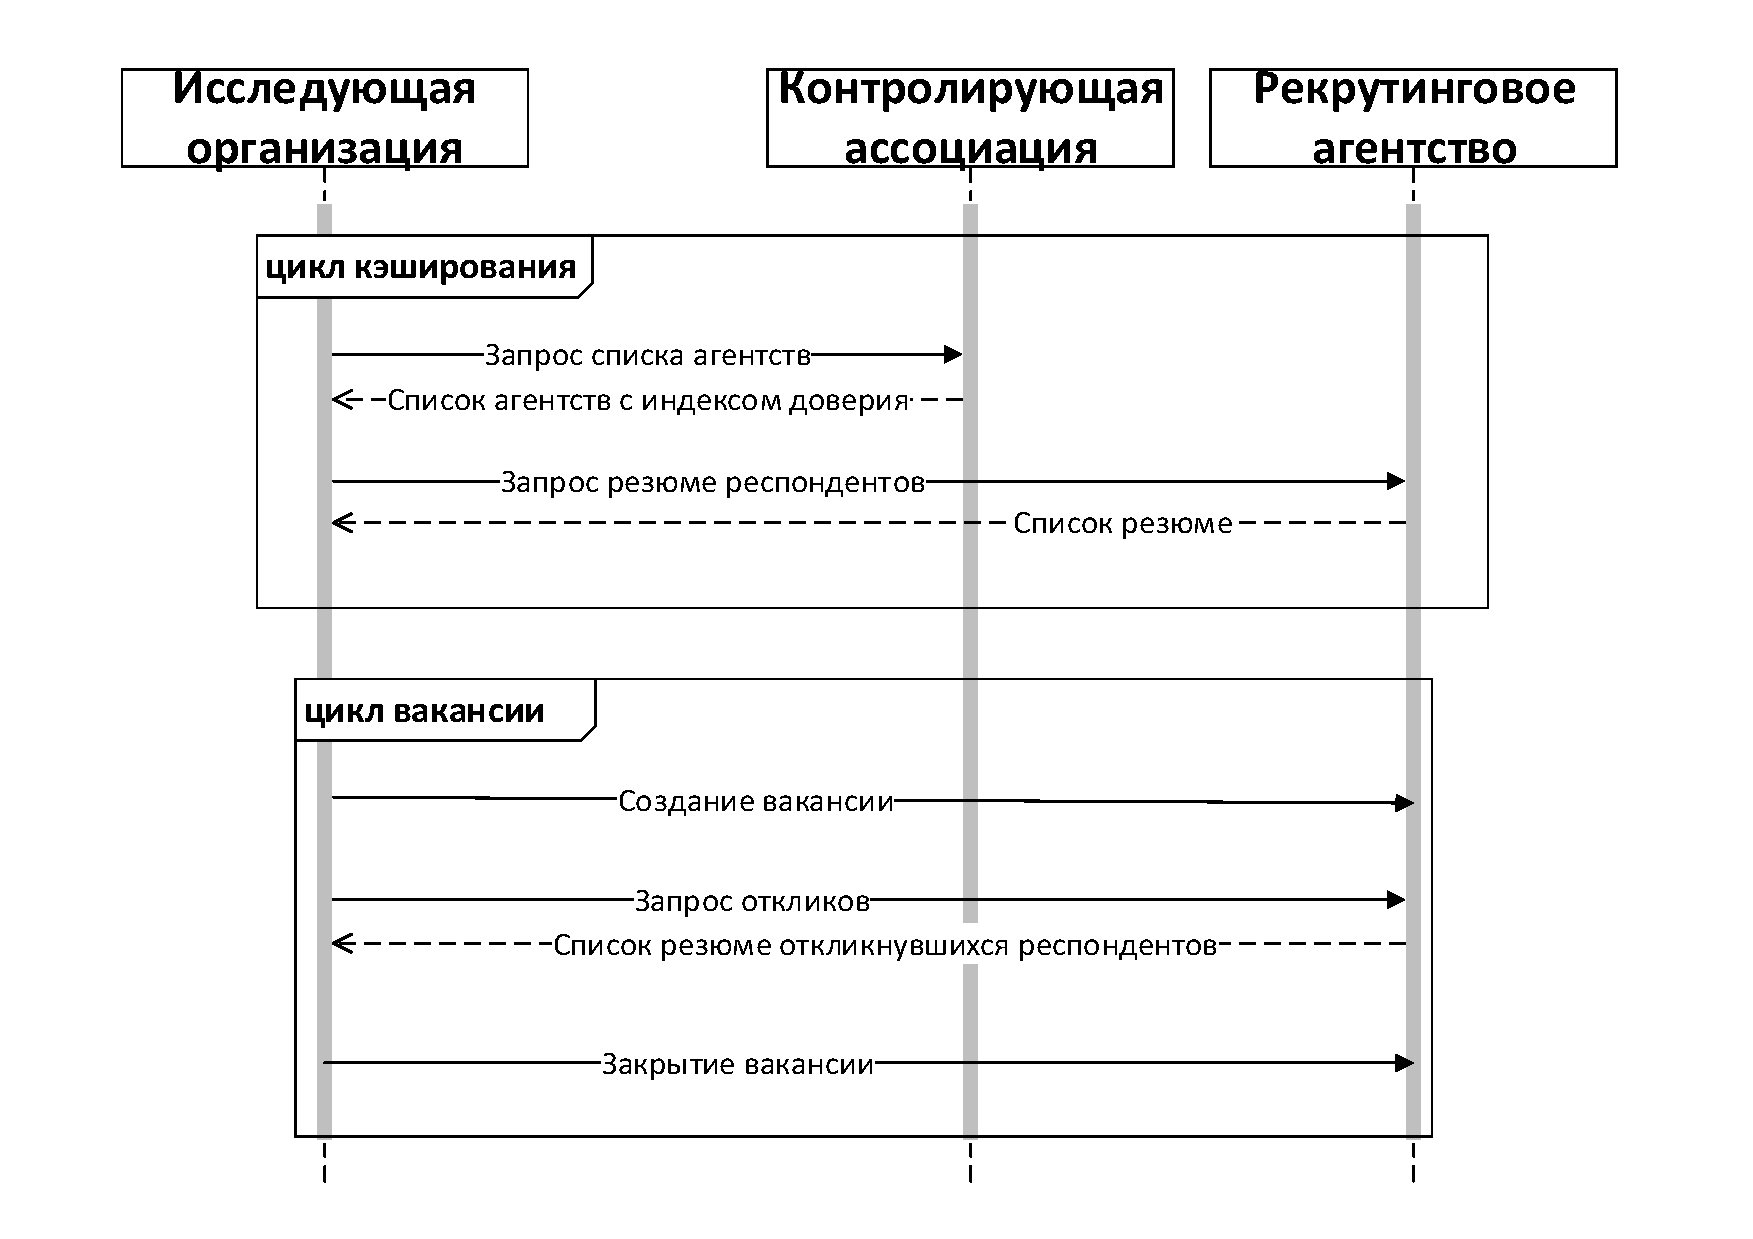
\includegraphics[width=\textwidth]{include/sequence1.pdf}
\caption{Диаграмма последовательности для подбора респондентов}
\label{fig:sequence1}
\end{figure}

\paragraph{Случай 2. Отправка отзыва и обновление рейтинга}

Периодически осуществляется кеширование списка рекрутинговых агентств. По запросу пользователя посылается асинхронный запрос с отзывом и оценкой конкретному агентству. После модерации отзыва в контролирующей ассоциации обновляется рейтинг доверия указанной системе, который будет обновлен при следующем кешировании.  
Диаграмма последовательности для отправки отзыва показана на рисунке ~\ref{fig:sequence2}.

\begin{figure}[ht]
  \centering
  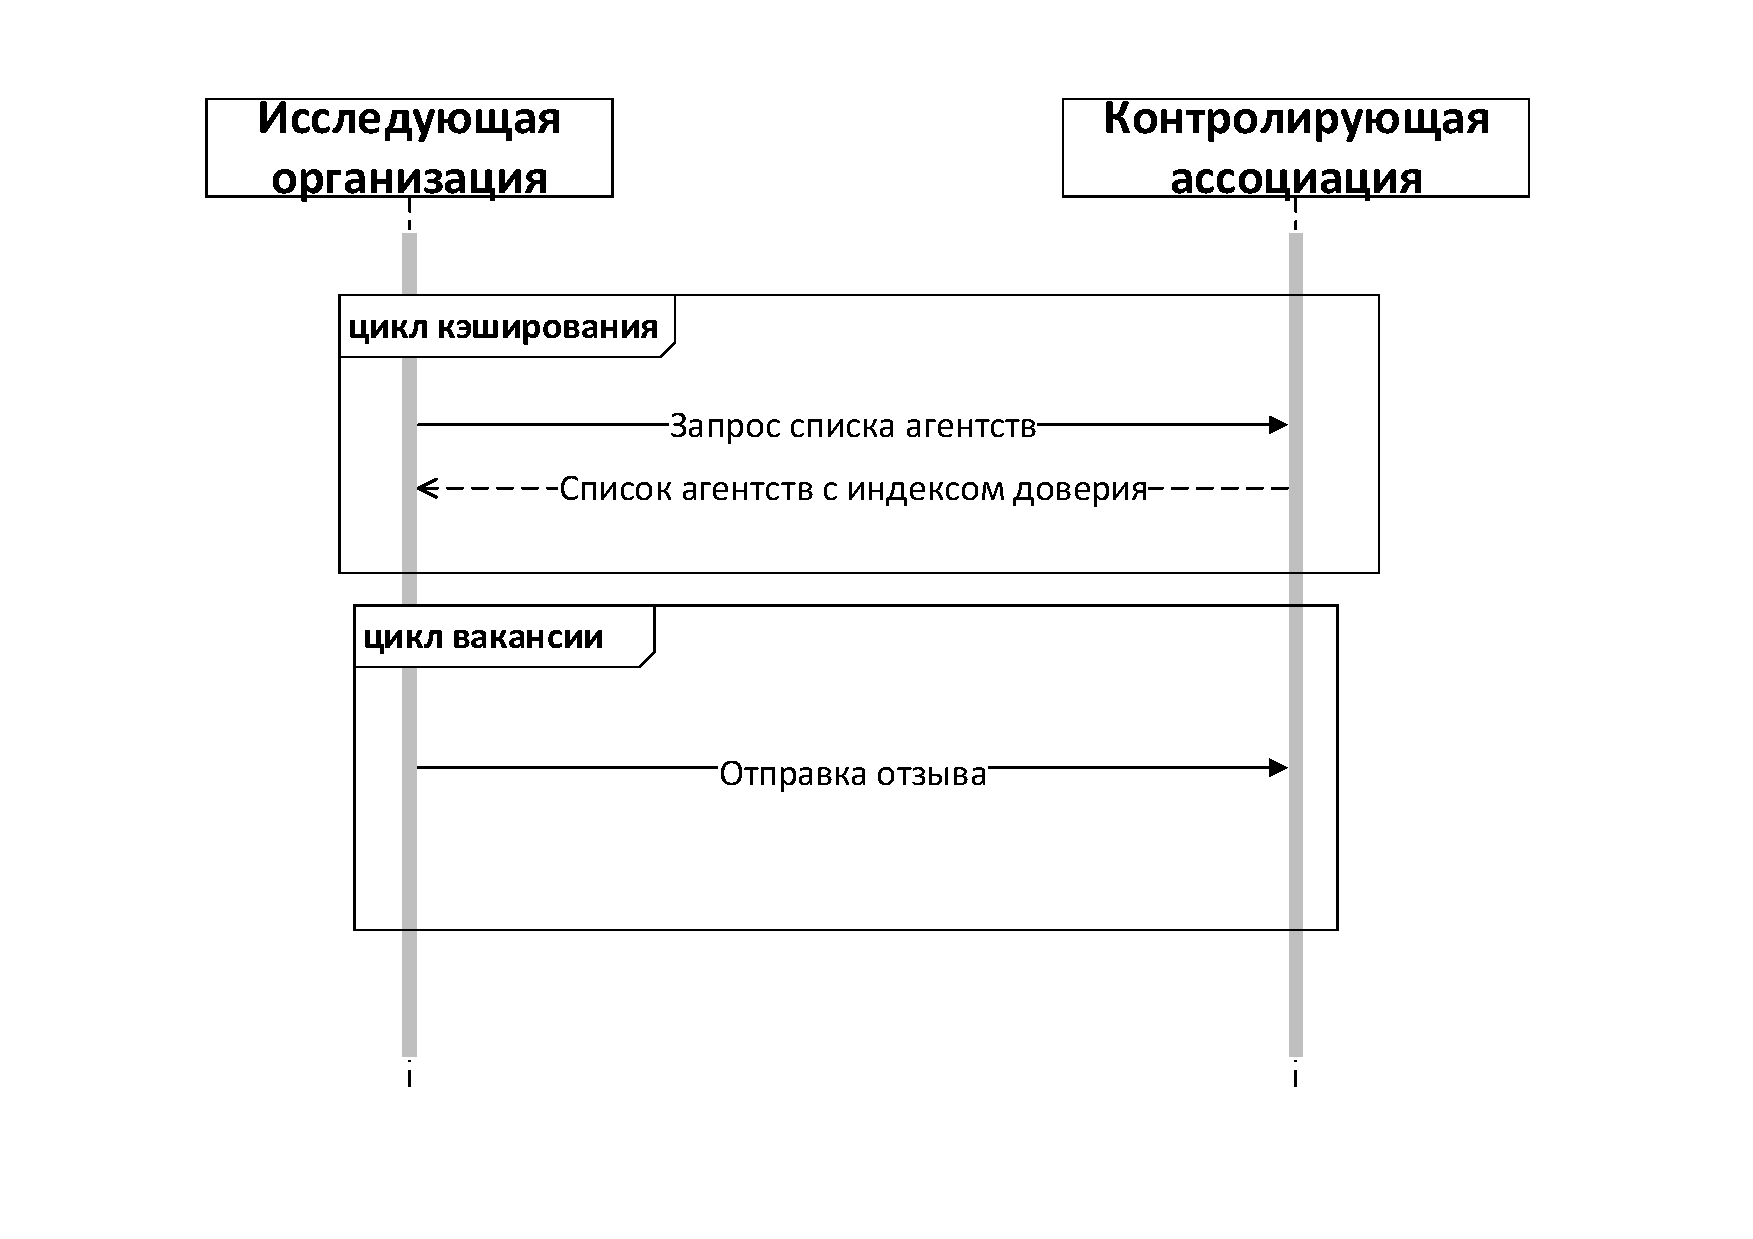
\includegraphics[width=\textwidth]{include/sequence2.pdf}
\caption{Диаграмма последовательности для отправки отзыва}
\label{fig:sequence2}
\end{figure}

\section{Система исследующей организации}
Данные системы исследующей организации содержат следующие сущности, связи которых представлены на рисунке ~\ref{fig:er-survey}, а описание атрибутов - на рисунке ~\ref{fig:er-survey-at}:

\begin{figure}[ht]
  \centering
  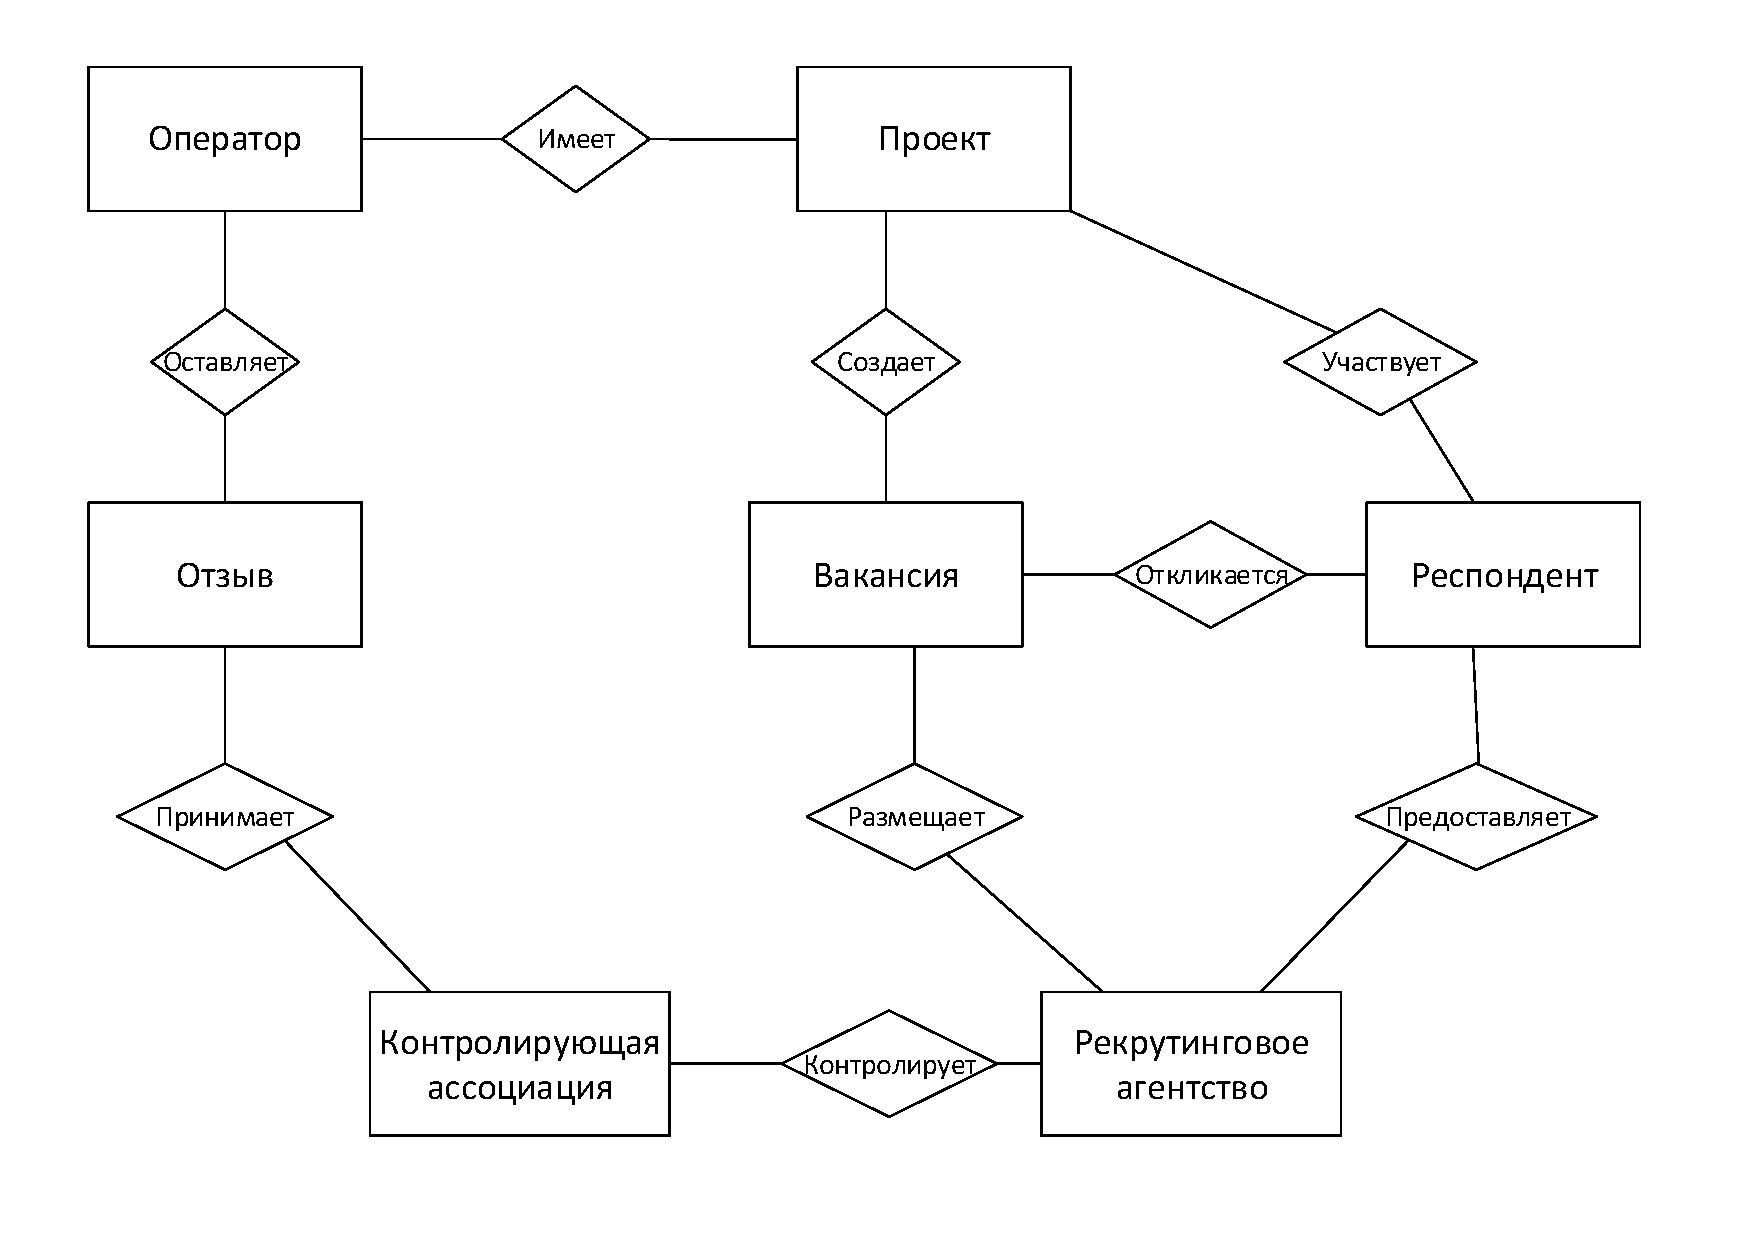
\includegraphics[width=\textwidth]{include/er-survey.pdf}
\caption{ER-диаграмма исследующей системы}
\label{fig:er-survey}
\end{figure}

\begin{figure}[ht]
  \centering
  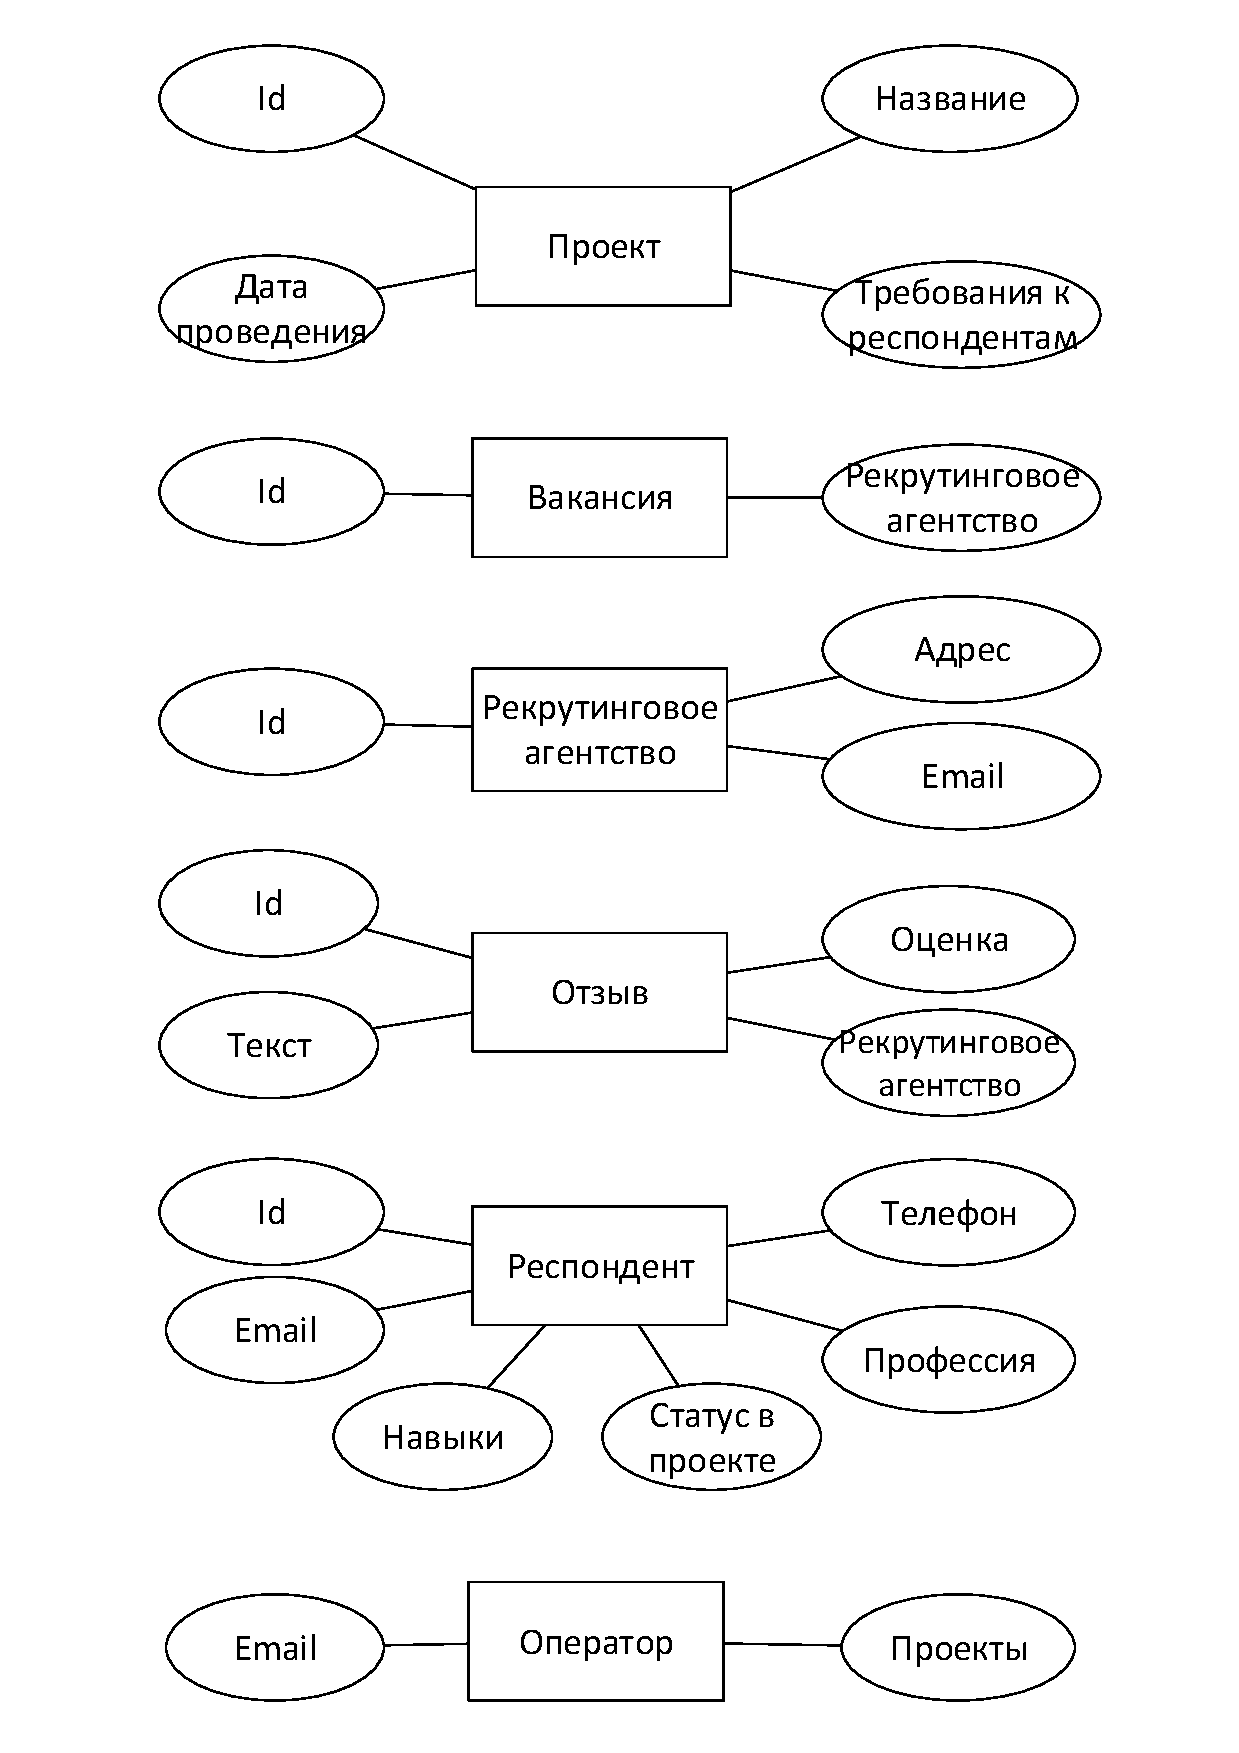
\includegraphics[width=\textwidth]{include/er-survey-at.pdf}
\caption{Атрибуты сущностей исследующей системы}
\label{fig:er-survey-at}
\end{figure}

\begin{enumerate}
\item оператор — имеет email и отображаемое имя, создает проекты и оставляет отзывы к рекрутинговым агентствам;
\item проект — имеет название, дату проведение и требования к респондентам, создает вакансии;
\item вакансия — создается в конкретном рекрутинговом агентстве и имеет ассоциированный проект;
\item рекрутинговое агентство — имеет адрес и email, предоставляется контролирующей ассоциацией;
\item отзыв — текст, оценка и id рекрутингового агентства в контролирующей ассоциации;
\item респондент — имеет имя, фамилию, email, телефон, профессию, навыки; может участвовать в проектах, откликаться на вакансии.
\item 
\end{enumerate}

\section{Система контролирующей ассоциации}
Данные системы контролирущей ассоциации содержат следующие сущности, связи которых представлены на рисунке ~\ref{fig:er-survey}, а описание атрибутов - на рисунке ~\ref{fig:er-survey-at}:

\begin{figure}[ht]
  \centering
  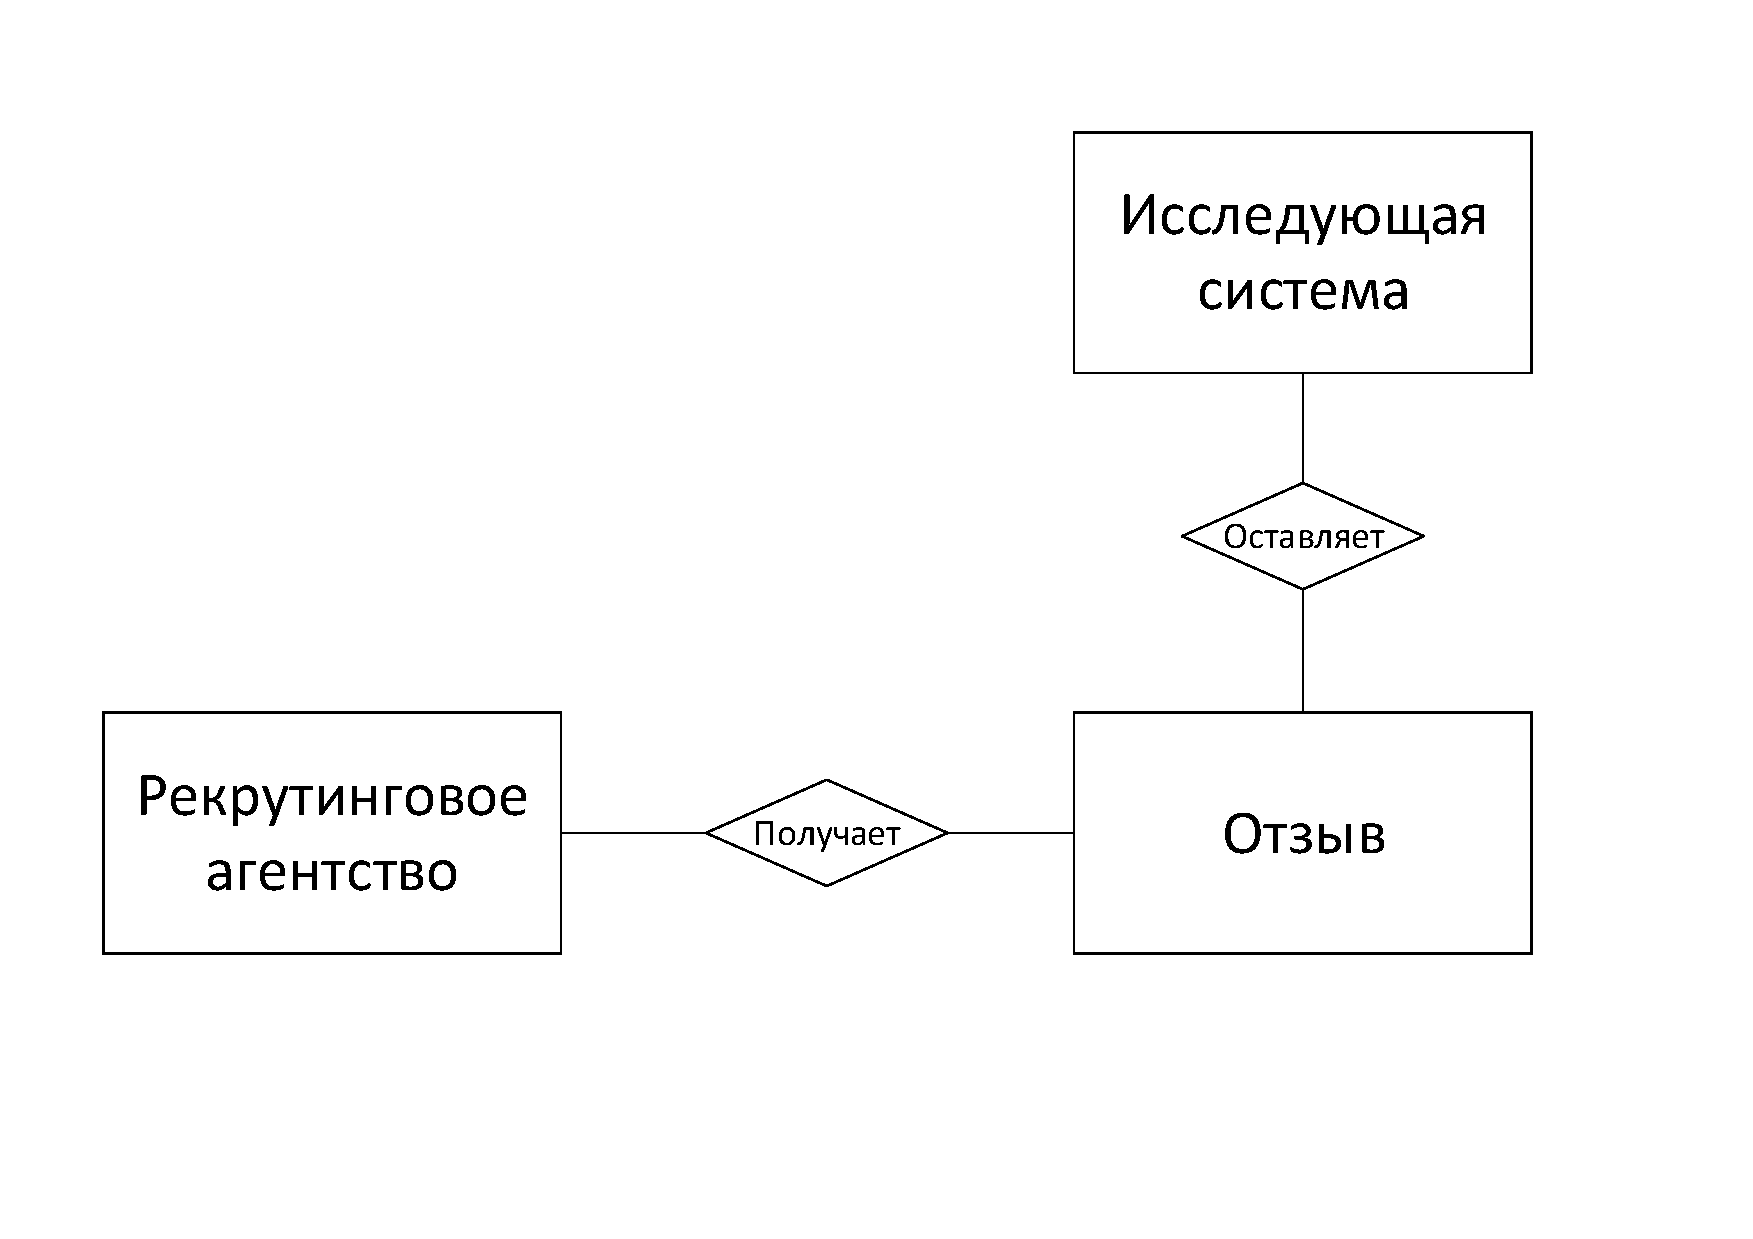
\includegraphics[width=\textwidth]{include/er-supervising.pdf}
\caption{ER-диаграмма контролирующей системы}
\label{fig:er-supervising}
\end{figure}

\begin{figure}[ht]
  \centering
  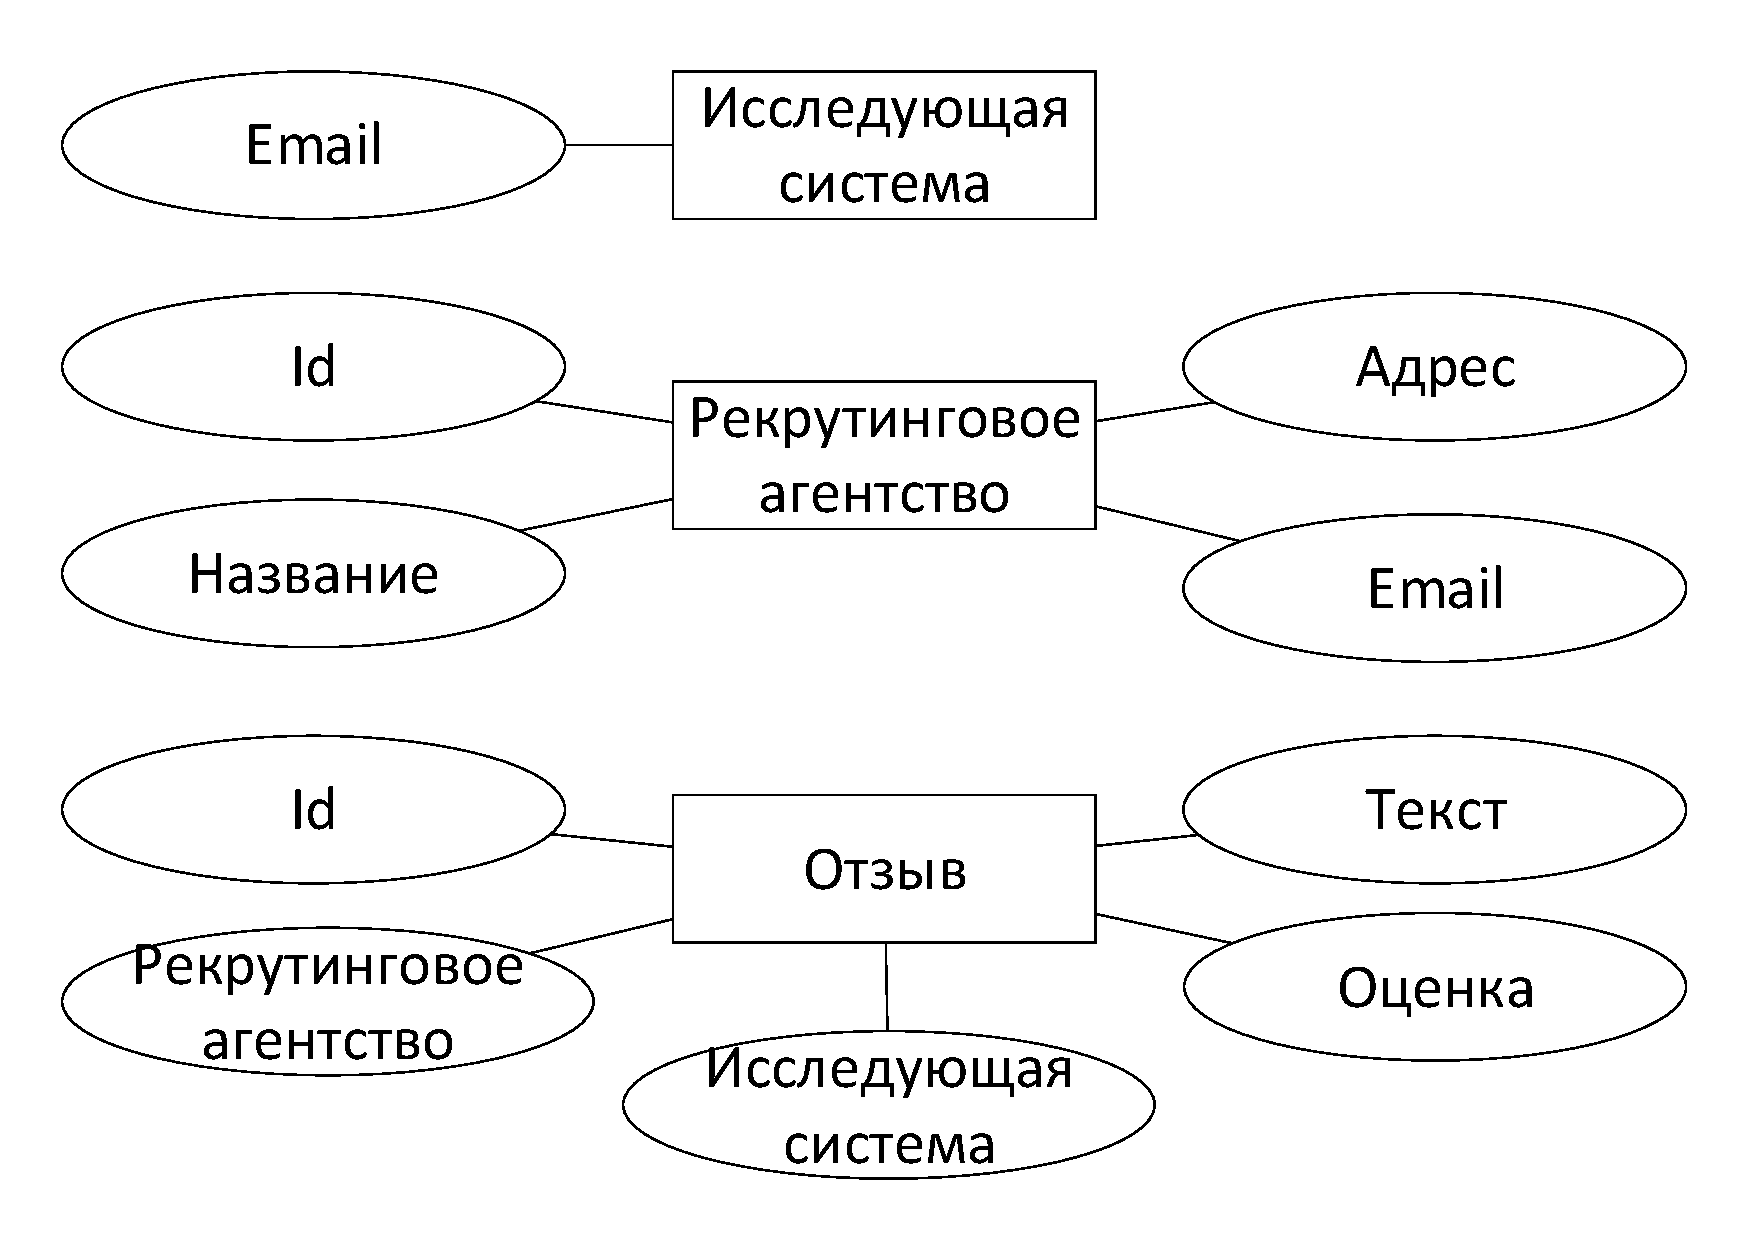
\includegraphics[width=\textwidth]{include/er-supervising-at.pdf}
\caption{Атрибуты сущностей контролирующей системы}
\label{fig:er-supervising-at}
\end{figure}

\begin{enumerate}
\item исследующая система — имеют email, оставляют отзывы;
\item рекрутинговое агентство — имеет название, адрес и email;
\item отзыв — имеет текст и оценку, оставляется исследующим агентством, относится к рекрутинговому агентству.
\end{enumerate}

\section{Система рекрутингового агентства}
Данные системы рекрутингового агентства содержат следующие сущности, связи которых представлены на рисунке ~\ref{fig:er-recruiting}, а описание атрибутов - на рисунке ~\ref{fig:er-recruiting-at}:

\begin{figure}[ht]
  \centering
  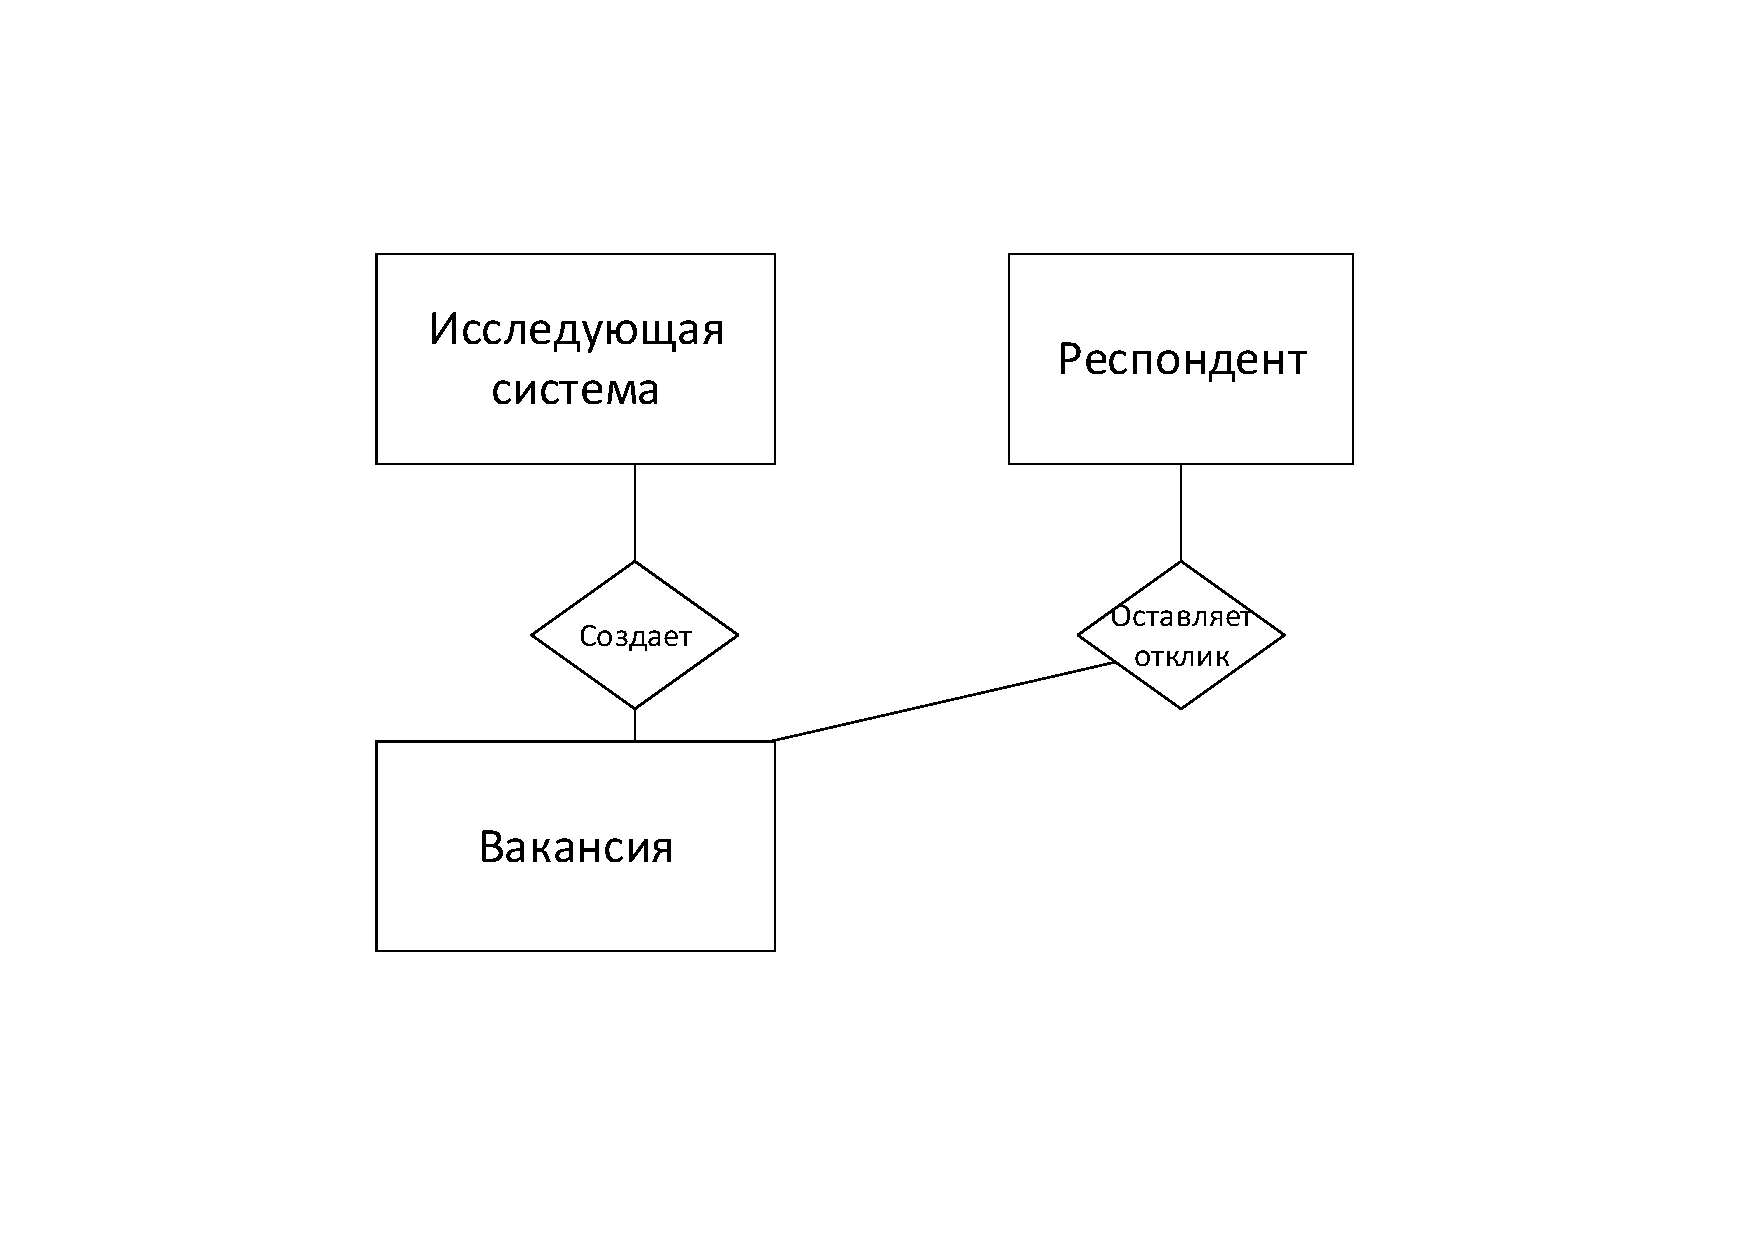
\includegraphics[width=\textwidth]{include/er-recruiting.pdf}
\caption{ER-диаграмма рекрутингового агентства}
\label{fig:er-recruiting}
\end{figure}

\begin{figure}[ht]
  \centering
  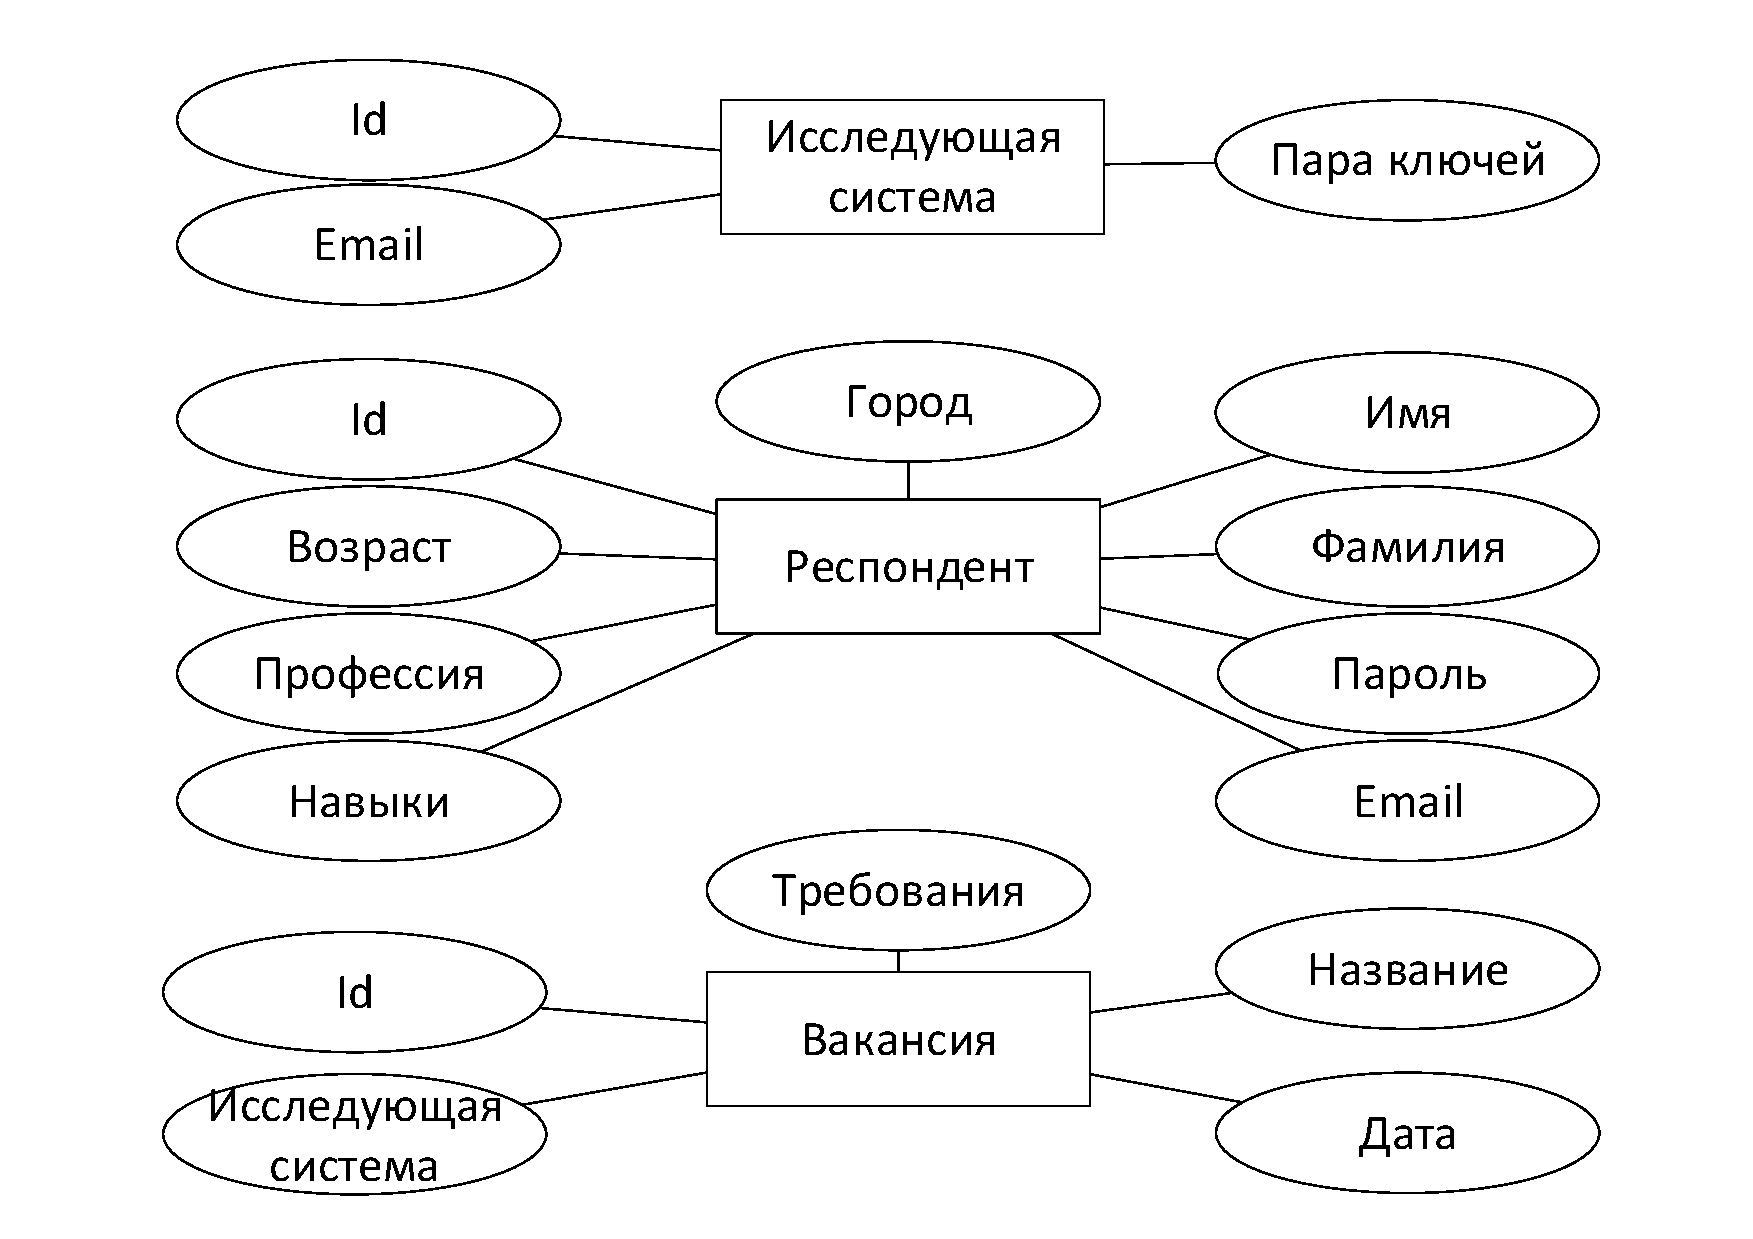
\includegraphics[width=\textwidth]{include/er-recruiting-at.pdf}
\caption{Атрибуты сущностей рекрутингового агентства}
\label{fig:er-recruiting-at}
\end{figure}

\begin{enumerate}
\item респондент — имеет такие атрибуты, как имя, фамилию, возраст, профессию, город, где он проживает, ключевые навыки, email и пароль к хэшированном виде; может оставлять отклики на вакансию;
\item вакансия — имеет название, дату, требования к респондентам;
\item исследующая организация — имеет email и пару ключей для подписи запросов; может создавать и закрывать вакансии;
\end{enumerate}

\subsection{Требования к шифрованию и цифровой подписи}
В рамках рассматриваемой работы сообщения должны передаваться по защищенным протоколам (HTTPS, SMTP+SSL). Сообщения в рекрутинговые агентства должны быть подписаны с помощью заранее заданного в конфигурации ключа.

%%% Local Variables:
%%% mode: latex
%%% TeX-master: "rpz"
%%% End:
